% Provenance (never printed): old seconde/premiere S material on water as a
% resource (stocks and flows of the water cycle, residence times, groundwater,
% overuse as a physical fact); see sources/book2/PROVENANCE.md. Residence
% times are computed in figdata/grade-10/residence_times.py, the Aral Sea
% budget in figdata/grade-10/aral_sea.py.
\chapter{Sumber Daya Air Tawar}\label{ch:g10:freshwater-resources}

Pada tahun 1960 Laut Aral, di gurun-gurun Asia Tengah, adalah danau terbesar
keempat di dunia. Dua sungai besar, yang dipasok oleh salju dan hujan di
pegunungan yang jauh, mengalir ke dalamnya; tidak ada yang mengalir keluar.
Pada tahun 1960-an air kedua sungai itu diambil untuk mengairi gurun. Satelit
telah mengamati apa yang terjadi sesudahnya: danau itu telah terpecah-pecah,
dan sebagian besar dasarnya kini menjadi daratan kering. Penyebabnya, sebagian
besar, bukanlah perubahan iklim, melainkan irigasi: danau itu menerima air
jauh lebih sedikit daripada yang diambil penguapan darinya setiap tahun. Bab
ini menghitung air di Bumi, di mana air itu tersimpan dan seberapa cepat air
itu bergerak, dan memperlihatkan bahwa sumber daya air terutama adalah sebuah
aliran: bila lebih banyak air diambil dari sebuah reservoir daripada yang
mengalir masuk ke dalamnya, reservoir itu mengosong, dengan laju yang dapat
diramalkan oleh neraca sederhana.
% ledger: nasa:aral, gaybullaev:aral-1960, micklin:aral

\begin{omfigure}
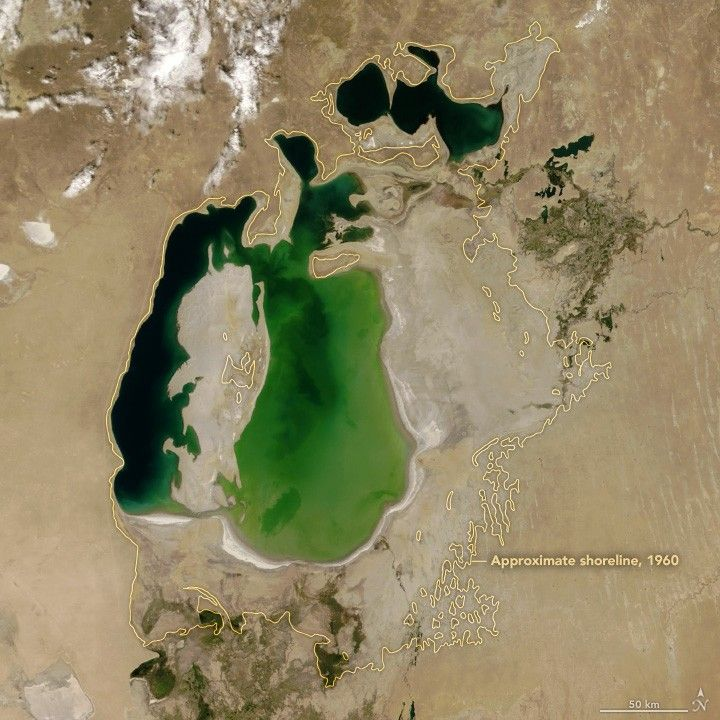
\includegraphics[width=0.47\linewidth]{images/book2/g10-nasa-aral-2000.jpg}\hspace{0.03\linewidth}%
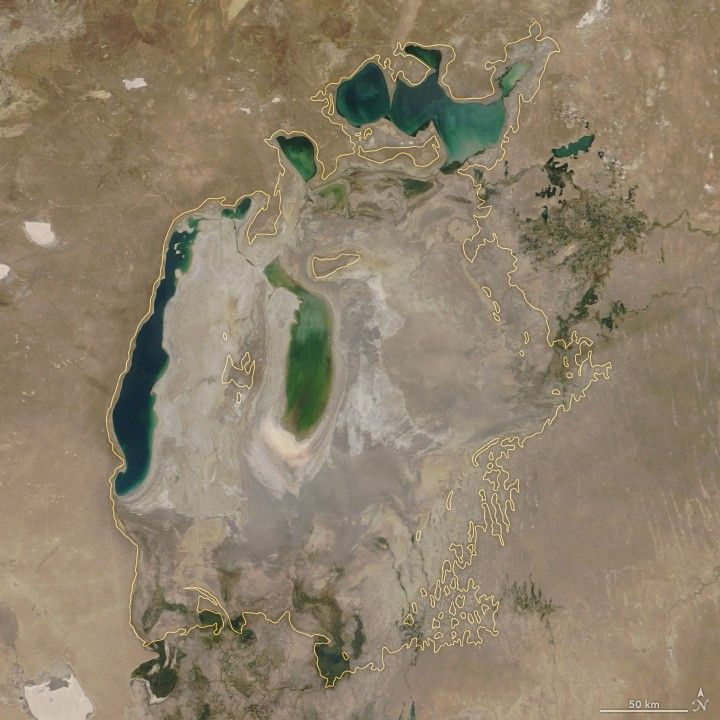
\includegraphics[width=0.47\linewidth]{images/book2/g10-nasa-aral-2018.jpg}

{\small Laut Aral dilihat oleh instrumen MODIS pada satelit Terra milik NASA
pada Agustus 2000 (kiri) dan Agustus 2018 (kanan); garis kuning adalah garis
pantai tahun 1960 secara kira-kira. Batang skalanya \qty{50}{km}. Citra: NASA
Earth Observatory.}
\end{omfigure}

\begin{recall}
Daur air memindahkan air di antara samudra, udara, dan daratan: penguapan,
pengembunan menjadi awan, presipitasi, air larian; massa total air kekal
(buku-buku fisika). Batuan yang pori-porinya saling terhubung bersifat
permeabel; di bawah muka air tanah pori-porinya penuh air, dan lapisan yang
menampung dan meloloskan cukup air untuk memasok sumur adalah akuifer (Buku 1,
kelas 6). Sebagian besar air di Bumi adalah air asin (Buku 1, kelas 2). Sungai
membawa pergi air dari daerah alirannya; \omterm{def:g10:drainage-basins:discharge}{debitnya} adalah volume per detik
(\cref{ch:g10:drainage-basins}).
\end{recall}

\section{Di mana air berada}

Bumi menyimpan sekitar 1.39 miliar kilometer kubik air. Hampir semuanya
berada di samudra; hanya \qty{2.5}{\percent} yang tawar. Dan sebagian besar air
tawar itu berada di luar jangkauan: lebih dari dua pertiganya membeku dalam
tudung es dan gletser, dan hampir sepertiganya terletak di bawah tanah.
% ledger: usgs:water-stocks

\begin{center}
\small
\begin{tabular}{|l|r|r|}
\hline
\textbf{reservoir} & \textbf{volume (\unit{km^3})} & \textbf{bagian dari air tawar} \\ \hline
samudra, laut, dan teluk & \num{1338000000} & (asin) \\ \hline
tudung es, gletser, dan salju abadi & \num{24064000} & \qty{68.7}{\percent} \\ \hline
air tanah tawar & \num{10530000} & \qty{30.1}{\percent} \\ \hline
es tanah dan permafrost & \num{300000} & \qty{0.86}{\percent} \\ \hline
danau air tawar & \num{91000} & \qty{0.26}{\percent} \\ \hline
kelembapan tanah & \num{16500} & \qty{0.05}{\percent} \\ \hline
atmosfer & \num{12900} & \qty{0.04}{\percent} \\ \hline
sungai & \num{2120} & \qty{0.006}{\percent} \\ \hline
\end{tabular}

{\small Salah satu perkiraan air di dunia, menurut Shiklomanov (1993), dari
U.S. Geological Survey. Air tanah asin (\num{12870000}~\unit{km^3}) dan danau
air asin tidak dimasukkan.}
\end{center}
% ledger: usgs:water-stocks

Sungai dan danau air tawar, tempat manusia mengambil sebagian besar air yang
dipakainya, bersama-sama menampung kurang dari seperseratus persen dari
seluruh air. Namun sungai tidak pernah lama mengering: sungai bukanlah
simpanan, melainkan aliran, yang diisi kembali oleh setiap hujan.

\section{Stok dan fluks}

\begin{definition}[Stok; fluks]\label{def:g10:freshwater-resources:stock}
Dalam neraca air, yang disebut \emph{stok}\index{stok (air)} adalah jumlah air
yang tersimpan dalam sebuah reservoir --- samudra, udara, es, akuifer, danau
--- pada suatu waktu, sebagai volume atau massa. Yang disebut
\emph{fluks}\index{fluks (air)} adalah jumlah yang berpindah dari satu
reservoir ke reservoir lain per satuan waktu, misalnya dalam kilometer kubik
per tahun.
\end{definition}

\omterm{def:g10:freshwater-resources:stock}{Stok} hanya berubah melalui \omterm{def:g10:freshwater-resources:stock}{fluks-fluksnya}: yang masuk dikurangi yang keluar.
Bila keduanya sama, \omterm{def:g10:freshwater-resources:stock}{stok} itu berada dalam \emph{keadaan tunak}: \omterm{def:g10:freshwater-resources:stock}{stok} itu tetap
sama meskipun airnya terus-menerus diganti.

\begin{omfigure}
\begin{tikzpicture}[font=\footnotesize, >={Stealth[length=6pt]}]
  % ocean, land, atmosphere
  \fill[omSea] (0,0) rectangle (6.4,1.6);
  \fill[omLithAlluv] (6.4,0) -- (6.4,1.6) -- (8.2,2.1) -- (10.4,2.6) -- (12,2.9) -- (12,0) -- cycle;
  \fill[omLithSand!60] (6.4,0) -- (12,0) -- (12,1.0) -- (6.4,0.7) -- cycle;
  \draw[black!50] (6.4,1.6) -- (8.2,2.1) -- (10.4,2.6) -- (12,2.9);
  \fill[omIce] (10.6,2.65) -- (11.3,3.35) -- (12,2.9) -- cycle;
  \node[align=center] at (3.2,0.75) {\textbf{samudra}\\\num{1335040}};
  \node[align=center] at (9.3,1.35) {kelembapan tanah 122\\danau dan sungai 178};
  \node[align=center] at (9.3,0.35) {air tanah \num{15300}};
  \node[align=center] at (11.2,2.25) {es\\\num{26350}};
  % atmosphere
  \draw[black!30, rounded corners=8pt, fill=omWxCloud] (1.0,4.6) rectangle (11.0,5.6);
  \node[align=center] at (6.0,5.1) {\textbf{atmosfer} 12.7};
  % fluxes
  \draw[->, omProp, line width=1.4pt] (1.4,1.7) -- node[left, align=right] {penguapan\\413} (1.4,4.5);
  \draw[->, omWxRain, line width=1.4pt] (4.4,4.5) -- node[pos=0.3, right, align=left] {presipitasi\\373} (4.4,1.7);
  \draw[->, omWxRain, line width=1.4pt] (7.6,4.5) -- node[pos=0.7, left, align=right] {presipitasi\\113} (7.6,2.05);
  \draw[->, omProp, line width=1.4pt] (10.0,2.6) -- node[right, align=left] {penguapan dan\\transpirasi 73} (10.0,4.5);
  \draw[->, black!60, line width=1.2pt] (4.9,5.85) -- node[above] {uap air yang dibawa ke atas daratan: 40} (7.4,5.85);
  \draw[->, omRiver, line width=1.4pt] (7.6,1.2) -- node[above, inner sep=2pt] {air larian 40} (6.0,1.2);
\end{tikzpicture}

{\small Daur air global pada tahun 1990-an (skematis; tidak berskala). \omterm{def:g10:freshwater-resources:stock}{Stok}
dalam ribuan \unit{km^3}, \omterm{def:g10:freshwater-resources:stock}{fluks} dalam ribuan \unit{km^3} per tahun. Menurut
Trenberth dan kawan-kawan (2007). Perkiraan \omterm{def:g10:freshwater-resources:stock}{stok} berbeda dari satu penelitian
ke penelitian lain: bandingkan air tanah dan es di sini dengan tabel di atas.}
\end{omfigure}
% ledger: trenberth:water-cycle

Daur itu seimbang. Setiap tahun samudra kehilangan \num{413000}~\unit{km^3}
melalui penguapan dan menerima kembali \num{373000} sebagai hujan dan salju
serta \num{40000} dari sungai-sungai. Udara menerima
$413\,000 + 73\,000 = \num{486000}$~\unit{km^3} dan mengembalikan
$373\,000 + 113\,000$, jumlah yang sama. Daratan menerima
\num{113000}~\unit{km^3} presipitasi; \num{73000} kembali ke udara melalui
penguapan dan melalui daun-daun tumbuhan, dan \num{40000} sisanya mengalir ke
laut, di sungai-sungai dan di bawah tanah.
% ledger: trenberth:water-cycle

\begin{definition}[Air tawar terbarukan]\label{def:g10:freshwater-resources:renewable}
Yang disebut \emph{air tawar terbarukan}\index{air tawar terbarukan} sebuah
wilayah adalah \omterm{def:g10:freshwater-resources:stock}{fluks} air tawar yang diperbarui setiap tahun oleh presipitasi,
yang mengalir melaluinya sebagai air larian di sungai dan sebagai air tanah.
Air tawar terbarukan adalah \omterm{def:g10:freshwater-resources:stock}{fluks}, dalam kilometer kubik per tahun, bukan
\omterm{def:g10:freshwater-resources:stock}{stok}.
\end{definition}

Untuk seluruh daratan Bumi, \omterm{def:g10:freshwater-resources:renewable}{air tawar terbarukan} adalah \num{40000}~\unit{km^3}
yang mencapai laut setiap tahun. Sebuah wilayah dapat memakai air
terbarukannya tahun demi tahun tanpa kekurangan. Apa yang diambilnya melebihi
jumlah itu hanya dapat berasal dari \omterm{def:g10:freshwater-resources:stock}{stok}, yang kemudian menyusut.

\section{Waktu tinggal}

Berapa lama sebuah molekul air tinggal dalam sebuah reservoir? Sebagian
langsung pergi, sebagian lain tinggal jauh lebih lama; tetapi secara
rata-rata, jawabannya hanya bergantung pada \omterm{def:g10:freshwater-resources:stock}{stok} dan \omterm{def:g10:freshwater-resources:stock}{fluks}.

\begin{definition}[Waktu tinggal]\label{def:g10:freshwater-resources:residence-time}
Yang disebut \emph{waktu tinggal}\index{waktu tinggal} air dalam sebuah
reservoir adalah waktu rata-rata yang dihabiskan air di dalamnya di antara saat
masuk dan saat keluar.
\end{definition}

\begin{proposition}[Waktu tinggal, stok, dan fluks]\label{prop:g10:freshwater-resources:residence}
Untuk reservoir dalam keadaan tunak, yang menyimpan \omterm{def:g10:freshwater-resources:stock}{stok} $S$ dan dilintasi
\omterm{def:g10:freshwater-resources:stock}{fluks} $F$ (masuk dan keluar), \omterm{def:g10:freshwater-resources:residence-time}{waktu tinggalnya} adalah
\[
T = \frac{S}{F}.
\]
\end{proposition}

\begin{proof}
Dalam keadaan tunak, volume $F$ masuk dan volume $F$ keluar setiap tahun,
sementara \omterm{def:g10:freshwater-resources:stock}{stoknya} tetap $S$. Setelah waktu $S/F$, volume $F \times S/F = S$
telah masuk: sebanyak yang ditampung seluruh reservoir. Secara rata-rata, air
yang ada pada awalnya kemudian telah diganti, sehingga air tinggal selama $S/F$
di dalam reservoir itu.
\end{proof}

\begin{example}[Air di udara]\label{ex:g10:freshwater-resources:atmosphere}
Atmosfer menyimpan \num{12700}~\unit{km^3} air, dan \num{486000}~\unit{km^3}
jatuh darinya setiap tahun sebagai hujan dan salju. \omterm{def:g10:freshwater-resources:residence-time}{Waktu tinggalnya}
$12\,700/486\,000 \approx \num{0.026}$ tahun, sekitar \num{9.5} hari: air di
udara diperbarui setiap satu atau dua minggu. Awan yang menurunkan hujan hari
ini tersusun atas air yang meninggalkan samudra atau tanah beberapa hari yang
lalu.
\end{example}
% ledger: trenberth:water-cycle (t_atmosphere_days 9.5 in figdata/grade-10/residence_times.py)

Perhitungan yang sama memberikan sekitar \num{19} hari untuk air di alur
sungai ($2120$~\unit{km^3} yang diangkut oleh \num{40000}~\unit{km^3}
setahun), beberapa tahun untuk danau dan sungai bersama-sama, dan sekitar
\num{3200} tahun untuk samudra ($1\,335\,040/413$ ribu~\unit{km^3}). Air
tanah dapat lebih lambat lagi: air terdalam di sebagian akuifer berumur
ratusan ribu tahun.
% ledger: trenberth:water-cycle, usgs:water-stocks, sturchio:nubian-age

\begin{omfigure}
\begin{tikzpicture}
\begin{axis}[omrecord, xbar, xmode=log, log origin=infty, width=0.74\linewidth, height=5.6cm,
  xmin=1, xmax=1e9, ymin=-0.6, ymax=4.6, bar width=11pt,
  ytick={0,1,2,3,4}, yticklabels={atmosfer, sungai, {danau dan sungai}, samudra, {air tanah dalam (umur)}},
  xtick={1,30.44,365.25,36525,3652500,365250000}, xticklabels={1 hari, 1 bulan, 1 tahun, 100 tahun, \num{10000} tahun, 1 juta tahun},
  xticklabel style={font=\scriptsize, rotate=25, anchor=north east}, yticklabel style={font=\small},
  xlabel={waktu tinggal (skala logaritmik)}, label style={font=\small}, xmajorgrids]
\addplot[fill=omDef!45, draw=omDef!80!black] table[x=days, y=idx] {figdata/out/grade-10-residence_times-times.dat};
\draw[fill=omProp!45, draw=omProp!80!black] (axis cs:73050000,3.75) rectangle (axis cs:365250000,4.25);
\node[anchor=west, font=\scriptsize] at (axis cs:9.5,0) {\num{9.5} hari};
\node[anchor=west, font=\scriptsize] at (axis cs:19.4,1) {\num{19} hari};
\node[anchor=west, font=\scriptsize] at (axis cs:1625,2) {\num{4.5} tahun};
\node[anchor=west, font=\scriptsize] at (axis cs:1180690,3) {\num{3200} tahun};
\node[anchor=east, font=\scriptsize] at (axis cs:73050000,4) {\num{200000} sampai 1 juta tahun};
\end{axis}
\end{tikzpicture}

{\small \omterm{def:g10:freshwater-resources:residence-time}{Waktu tinggal} air, dihitung sebagai \omterm{def:g10:freshwater-resources:stock}{stok} dibagi \omterm{def:g10:freshwater-resources:stock}{fluks} dari daur air
global (biru), dan umur terukur air tanah dalam di bawah Sahara timur
(jingga). Sumbu logaritmik: mulai dari satu tahun, setiap langkah yang
ditandai adalah seratus kali lipat. Data: Trenberth dan kawan-kawan (2007);
U.S. Geological Survey; Sturchio dan kawan-kawan (2004).}
\end{omfigure}
% values computed in figdata/grade-10/residence_times.py

\omterm{def:g10:freshwater-resources:residence-time}{Waktu tinggal} mengukur seberapa cepat sebuah reservoir pulih. Air yang diambil
dari sungai diganti dalam beberapa hari; danau yang tercemar atau dikosongkan
memerlukan bertahun-tahun; air tanah yang memerlukan ribuan tahun untuk
terkumpul, pada skala hidup manusia, sama sekali tidak diperbarui.

\begin{method}[Neraca air]\label{met:g10:freshwater-resources:budget}
\begin{enumerate}
  \item Pilih reservoirnya: danau, akuifer, \omterm{def:g10:drainage-basins:drainage-basin}{daerah aliran sungai}, udara.
  \item Daftarlah setiap \omterm{def:g10:freshwater-resources:stock}{fluks} yang masuk ke dalamnya (sungai, hujan,
        rembesan) dan yang keluar darinya (sungai, penguapan, pemompaan),
        dalam satuan yang sama.
  \item Perubahan \omterm{def:g10:freshwater-resources:stock}{stok} per tahun adalah jumlah masukan dikurangi jumlah
        keluaran.
  \item Jika \omterm{def:g10:freshwater-resources:stock}{stok} tidak berubah, masukan sama dengan keluaran, dan \omterm{def:g10:freshwater-resources:residence-time}{waktu
        tinggalnya} adalah \omterm{def:g10:freshwater-resources:stock}{stok} dibagi salah satunya.
\end{enumerate}
\end{method}

\section{Akuifer sebagai reservoir}

Hujan yang meresap ke dalam tanah dan mencapai muka air tanah
\emph{mengimbuh} akuifer di bawahnya. Air itu lalu bergerak perlahan melalui
pori-pori batuan, menuju mata air, sungai, atau laut. Di tempat lapisan
permeabel menyusup ke bawah lapisan kedap, seperti lempung, airnya menjadi
\emph{tertekan}: air itu hanya dipasok di tempat lapisan itu mencapai
permukaan, yang mungkin jauh letaknya.

\begin{omfigure}
\begin{tikzpicture}[font=\footnotesize, >={Stealth[length=5pt]}]
  % layers dipping to the right
  \fill[lith shale] (0,0) -- (12,0) -- (12,0.8) -- (0,2.4) -- cycle;
  \fill[lith sandstone] (0,2.4) -- (12,0.8) -- (12,2.2) -- (2.2,3.5) -- (0,3.8) -- cycle;
  \fill[lith shale] (2.2,3.5) -- (12,2.2) -- (12,3.4) -- (3.6,3.9) -- cycle;
  % ground surface
  \draw[line width=0.8pt, brown!60!black] (0,3.8) -- (1.2,4.0) -- (2.2,3.9) -- (3.6,3.9) -- (6,3.6) -- (9,3.5) -- (12,3.4);
  \fill[omLithAlluv] (0,3.8) -- (1.2,4.0) -- (2.2,3.9) -- (2.2,3.5) -- (0,3.8) -- cycle;
  \fill[omLithAlluv] (2.2,3.9) -- (3.6,3.9) -- (2.2,3.5) -- cycle;
  \fill[omLithAlluv] (3.6,3.9) -- (6,3.6) -- (9,3.5) -- (12,3.4) -- (3.6,3.9) -- cycle;
  % water table in the unconfined part
  \draw[omDef, line width=1pt, dashed] (0,3.3) .. controls (1.0,3.35) and (1.8,3.2) .. (2.6,3.45);
  \node[anchor=south west, text=omDef, fill=white, fill opacity=0.8, text opacity=1, inner sep=1pt] at (0.05,2.75) {muka air tanah};
  % rain and recharge
  \foreach \x in {0.35,0.65,0.95,1.25} \draw[omWxRain, thick] (\x,4.9) -- (\x-0.15,4.4);
  \node[anchor=south, text=omWxRain] at (0.7,4.95) {hujan: imbuhan};
  % flow arrows in the aquifer
  \draw[->, omDef, line width=1.1pt] (2.0,2.85) -- (4.4,2.55);
  \draw[->, omDef, line width=1.1pt] (5.4,2.4) -- (7.8,2.1);
  \draw[->, omDef, line width=1.1pt] (8.8,1.95) -- (11.2,1.65);
  % wells
  \draw[black!70, line width=1.6pt] (1.95,3.95) -- (1.95,2.9);
  \node[anchor=south] at (1.95,4.0) {sumur};
  \draw[black!70, line width=1.6pt] (7.0,3.55) -- (7.0,1.9);
  \node[anchor=south] at (7.0,3.6) {sumur};
  % labels
  \node[align=center, fill=white, fill opacity=0.85, text opacity=1, inner sep=1.5pt] at (1.5,0.8) {lempung kedap};
  \node[align=center, fill=white, fill opacity=0.85, text opacity=1, inner sep=1.5pt] at (8.6,2.95) {lempung kedap};
  \node[anchor=north, align=center] at (1.6,-0.1) {akuifer bebas:\\daerah imbuhan};
  \node[anchor=north, align=center] at (6.4,-0.1) {akuifer tertekan};
  \node[anchor=north, align=center] at (10.6,-0.1) {air tua, jauh dari\\daerah imbuhan};
\end{tikzpicture}

{\small Akuifer dalam batu pasir yang permeabel (skematis). Hujan
mengimbuhnya di tempat batu pasir itu mencapai permukaan; di sana muka air
tanah bebas naik dan turun. Lebih jauh, di bawah lempung, akuifer itu
tertekan, dan airnya bergerak perlahan menuruni lapisan: makin jauh dari
daerah imbuhan, makin tua airnya.}
\end{omfigure}

\begin{definition}[Air tanah fosil]\label{def:g10:freshwater-resources:fossil-groundwater}
Yang disebut \emph{air tanah fosil}\index{air tanah fosil} adalah air tanah
yang memasuki akuifernya sejak lama, sering kali di bawah iklim yang lebih
basah, dan yang tidak diperbarui oleh imbuhan masa kini pada skala hidup
manusia.
\end{definition}

Di bawah Sahara timur terbentang akuifer batu pasir yang sangat luas. Airnya
yang terdalam, yang ditentukan umurnya melalui peluruhan suatu bentuk
radioaktif kripton yang langka, berumur \num{200000} sampai satu juta tahun.
Air itu mengalir masuk perlahan dari daerah imbuhan di Mesir barat daya, dan
kimianya memperlihatkan bahwa air itu jatuh sebagai hujan selama masa-masa
basah pada zaman es, ketika udara lembap dari Atlantik mencapai wilayah itu.
Bila dipompa saat ini, air seperti itu adalah \omterm{def:g10:freshwater-resources:stock}{stok} yang sedang ditambang,
bukan aliran.
% ledger: sturchio:nubian-age

Bila pemompaan melebihi imbuhan, muka air tanah turun. Di High Plains di
Amerika Serikat bagian tengah, akuifer di bawah sekitar \num{175000} mil
persegi (\qty{453000}{km^2}) telah dipompa untuk irigasi sejak sekitar 1950.
Pada tahun 2015 muka airnya telah turun rata-rata \qty{4.8}{m}, dan sampai
\qty{71}{m} (234 kaki) di beberapa sumur; akuifer itu telah kehilangan sekitar
\num{273} juta ekar-kaki air, sekitar \qty{340}{km^3}.
% ledger: mcguire:high-plains (1 acre-foot = 1233.5 m3)

\begin{omfigure}
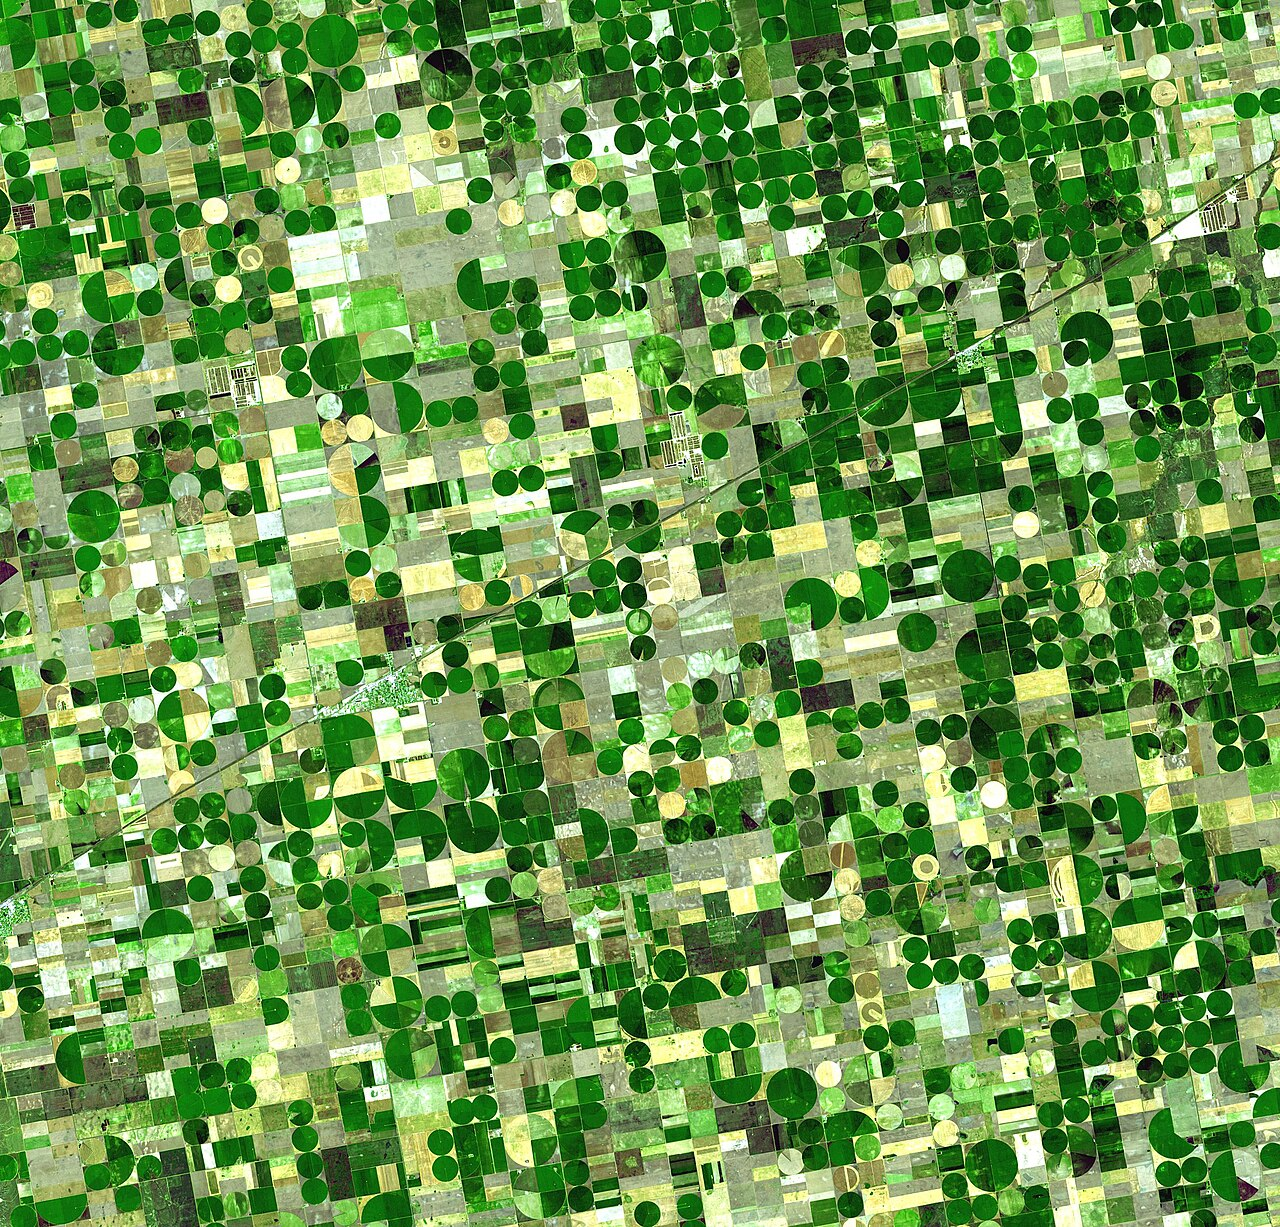
\includegraphics[width=0.5\linewidth]{images/book2/g10-nasa-kansas-center-pivot.jpg}

{\small Ladang-ladang beririgasi di dekat Sublette, Kansas, dilihat oleh
instrumen ASTER pada satelit Terra milik NASA pada Juni 2001 (lebarnya sekitar
\qty{37}{km}). Setiap lingkaran adalah ladang yang diairi oleh lengan
penyiram panjang yang berputar mengelilingi pusatnya; diameter
lingkaran-lingkaran itu \num{800} dan \qty{1600}{m}. Citra: NASA (domain
publik).}
\end{omfigure}

Air tanah tidak dapat dilihat dari angkasa, tetapi dapat ditimbang: dua
satelit yang terbang beriringan merasakan perubahan kecil tarikan Bumi yang
disebabkan oleh massa air yang datang dan pergi di bawahnya, dan memetakan di
mana \omterm{def:g10:freshwater-resources:stock}{stok} air di daratan naik dan turun dari bulan ke bulan.

\begin{omfigure}
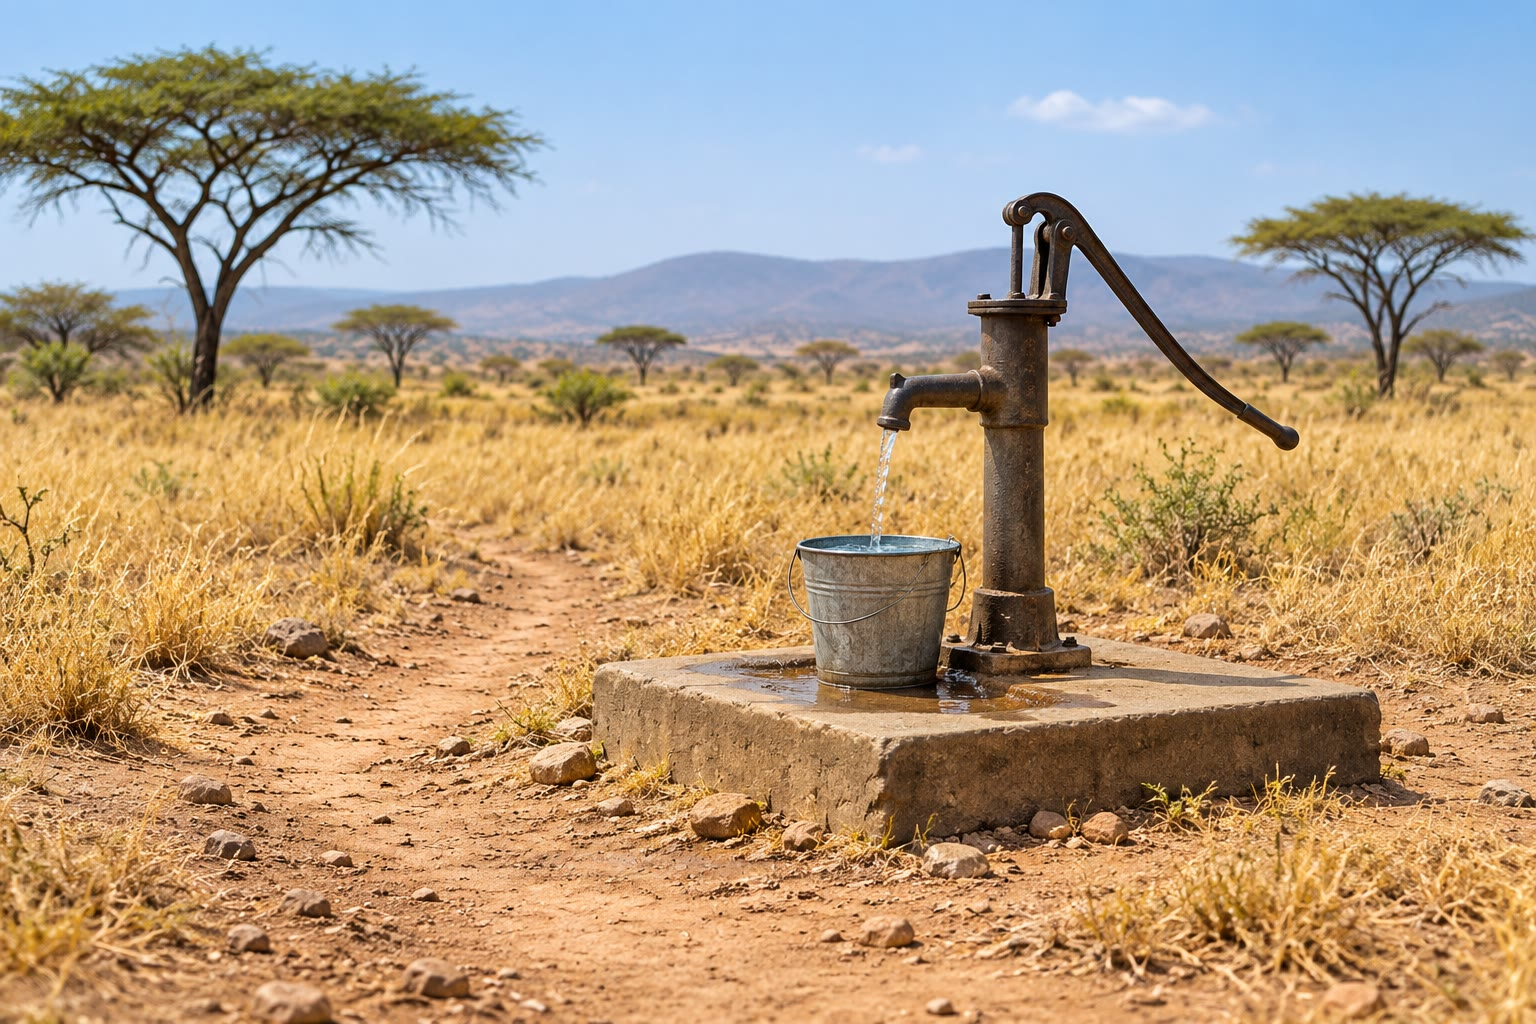
\includegraphics[width=0.55\linewidth]{images/book2/ai/g10-hand-pump-well.jpg}

{\small Pompa tangan pada sebuah sumur di bentang alam yang kering: air yang
diambil di sini berasal dari tanah di bawahnya, di luar jangkauan musim
kemarau.}
\end{omfigure}

\section{Penggunaan berlebihan sebagai fakta fisika}

Laut Aral tidak memiliki saluran keluar: air dari kedua sungainya, Amu Darya
dan Syr Darya, hanya pergi melalui penguapan. Pada tahun 1960 danau itu
meliputi \qty{68000}{km^2}, menampung \qty{1093}{km^3}, dan airnya mengandung
\qty{10}{g} garam per liter. Pada tahun itu penguapan mengambil
\qty{71.1}{km^3}, dan hujan di atas danau membawa \qty{9.4}{km^3}: untuk
mempertahankan muka airnya, danau itu memerlukan
$71.1 - 9.4 = \qty{61.7}{km^3}$ setahun dari sungai-sungainya.
% ledger: gaybullaev:aral-1960, gaybullaev:aral-table

Sejak tahun 1960-an sungai-sungai itu dialihkan untuk mengairi gurun, dan
hampir tidak ada airnya yang mencapai danau: pada tahun 1970-an dan 1980-an,
sering kali kurang dari \qty{2}{km^3} setahun. Penguapan terus berlangsung,
dan danau itu mulai menyusut. Neracanya menentukan seberapa cepat. Penguapan
mengambil lapisan air yang tebalnya bergantung pada iklim, di sini sekitar
satu meter setahun ($71.1/68\,000 \approx \qty{0.00105}{km}$). Jika aliran
masuk berhenti, muka air turun kira-kira sebesar itu setiap tahun, dikurangi
hujan. Ketika danau menyusut, luasnya dan karena itu juga penguapannya ikut
menyusut, dan penurunan itu melambat; tetapi penurunan itu tidak berhenti
sampai aliran masuk dan penguapan kembali seimbang.
% ledger: gaybullaev:aral-table (values computed in figdata/grade-10/aral_sea.py)

\begin{omfigure}
\begin{tikzpicture}
\begin{axis}[omrecord, name=vol, width=0.46\linewidth, height=5.4cm, xmin=1955, xmax=2012, ymin=0, ymax=1200,
  xtick={1960,1980,2000}, xticklabel style={/pgf/number format/1000 sep={}}, scaled y ticks=false,
  ylabel={volume (\unit{km^3})}, xlabel={tahun}, tick label style={font=\small}, label style={font=\small},
  title={\small volume air}]
\addplot[omDef, line width=1pt, mark=*, mark size=1.3pt] table[x=year, y=volume] {figdata/out/grade-10-aral_sea-record.dat};
\end{axis}
\begin{axis}[omrecord, at={(vol.east)}, anchor=west, xshift=1.4cm, width=0.46\linewidth, height=5.4cm,
  xmin=1955, xmax=2012, ymin=0, ymax=140, xtick={1960,1980,2000},
  xticklabel style={/pgf/number format/1000 sep={}},
  ylabel={salinitas (\unit{g/L})}, xlabel={tahun}, tick label style={font=\small}, label style={font=\small},
  title={\small salinitas}]
\addplot[omProp, line width=1pt, mark=*, mark size=1.3pt] table[x=year, y=salinity] {figdata/out/grade-10-aral_sea-record.dat};
\end{axis}
\end{tikzpicture}

{\small Laut Aral dari 1960 sampai 2010: volume airnya turun menjadi
sepersepuluh, sementara garam yang ditinggalkan penguapan menjadi tiga belas
kali lebih pekat. Data: Gaybullaev dan kawan-kawan (2012).}
\end{omfigure}
% ledger: gaybullaev:aral-table

Pada tahun 2010 danau itu menampung \qty{98}{km^3}, sepersepuluh volumenya
pada tahun 1960, di atas \qty{14280}{km^2}; salinitasnya telah mencapai
\qty{130}{g/L}, jauh lebih asin daripada samudra. Muka airnya telah turun
lebih dari \qty{20}{m}. Debu bergaram berembus dari dasar yang kering.
Penyebabnya tidak tersembunyi: aliran masuk danau itu diputus, sedangkan
penguapannya tidak.
% ledger: gaybullaev:aral-table, gaybullaev:aral-1960, micklin:aral, nasa:aral

\section{Latihan}

\begin{exercise}[$\star$]\label{exo:g10:freshwater-resources:1}
Definisikan \omterm{def:g10:freshwater-resources:stock}{stok}, \omterm{def:g10:freshwater-resources:stock}{fluks}, dan \omterm{def:g10:freshwater-resources:residence-time}{waktu tinggal}, lalu sebutkan satuan masing-masing.
\end{exercise}

\begin{exercise}[$\star$]\label{exo:g10:freshwater-resources:2}
Dari tabel air di dunia: berapa bagian dari seluruh air yang tawar? Dari air
tawar itu, berapa bagian yang membeku dan berapa yang berada di bawah tanah?
Reservoir manakah yang menampung paling sedikit?
\end{exercise}

\begin{exercise}[$\star$]\label{exo:g10:freshwater-resources:3}
Definisikan \omterm{def:g10:freshwater-resources:renewable}{air tawar terbarukan} dan \omterm{def:g10:freshwater-resources:fossil-groundwater}{air tanah fosil}. Mengapa yang pertama
adalah \omterm{def:g10:freshwater-resources:stock}{fluks} dan yang kedua adalah \omterm{def:g10:freshwater-resources:stock}{stok}?
\end{exercise}

\begin{exercise}[$\star$]\label{exo:g10:freshwater-resources:4}
Berapa kali lebih banyak air yang ditampung danau-danau air tawar di dunia
(\num{91000}~\unit{km^3}) dibandingkan dengan sungai-sungainya
(\num{2120}~\unit{km^3})?
\end{exercise}

\begin{exercise}[$\star$]\label{exo:g10:freshwater-resources:5}
Pada grafik \omterm{def:g10:freshwater-resources:residence-time}{waktu tinggal}, reservoir manakah yang memperbarui airnya paling
cepat, dan manakah yang paling lambat? Berapa kali lebih lama air tinggal di
samudra dibandingkan dengan di udara?
\end{exercise}

\begin{exercise}[$\star\star$]\label{exo:g10:freshwater-resources:6}
Atmosfer menyimpan \num{12700}~\unit{km^3} air. Hitung \omterm{def:g10:freshwater-resources:residence-time}{waktu tinggalnya} dari
penguapan yang memasukinya (\num{413000} dari samudra dan
\num{73000}~\unit{km^3} dari daratan setiap tahun), dan periksalah bahwa
hasilnya sesuai dengan \omterm{def:g10:freshwater-resources:residence-time}{waktu tinggal} yang dihitung dari presipitasi yang
keluar darinya.
\end{exercise}

\begin{exercise}[$\star\star$]\label{exo:g10:freshwater-resources:7}
Samudra menyimpan \num{1335040} ribu~\unit{km^3} dan kehilangan
\num{413} ribu~\unit{km^3} setahun melalui penguapan. Hitung \omterm{def:g10:freshwater-resources:residence-time}{waktu tinggalnya}.
Mengapa hasilnya sama jika dihitung dengan apa yang masuk ke dalamnya?
\end{exercise}

\begin{exercise}[$\star\star$]\label{exo:g10:freshwater-resources:8}
Dengan \omterm{def:g10:freshwater-resources:stock}{fluks-fluks} daur air global, tuliskan neraca daratan: apa yang jatuh
di atasnya, apa yang kembali ke udara, apa yang mengalir pergi. Berapa bagian
hujan yang jatuh di daratan yang kembali ke udara?
\end{exercise}

\begin{exercise}[$\star\star$]\label{exo:g10:freshwater-resources:9}
Akuifer High Plains kehilangan sekitar \num{273.2} juta ekar-kaki air dari
sekitar 1950 sampai 2015 (\num{1}~ekar-kaki = \qty{1233.5}{m^3}). Ubahlah
volume ini ke \unit{km^3} dan bandingkan dengan volume Laut Aral pada tahun
1987 (\qty{345.6}{km^3}).
\end{exercise}

\begin{exercise}[$\star\star$]\label{exo:g10:freshwater-resources:10}
Muka air rata-rata akuifer High Plains turun \num{15.8} kaki dari sekitar 1950
sampai 2015 (\num{1}~kaki = \qty{0.3048}{m}). Berapa itu dalam meter, dan dalam
sentimeter per tahun?
\end{exercise}

\begin{exercise}[$\star\star$]\label{exo:g10:freshwater-resources:11}
Sebuah akuifer menyimpan \qty{2}{km^3} air dan diimbuh \qty{0.01}{km^3}
setahun. Berapa \omterm{def:g10:freshwater-resources:residence-time}{waktu tinggal} airnya? Sumur-sumur kini memompa
\qty{0.05}{km^3} setahun darinya. Misalkan imbuhan terus berlangsung dan
sumur-sumur kini menjadi satu-satunya jalan keluar bagi air itu: berapa lama
air itu akan bertahan?
\end{exercise}

\begin{exercise}[$\star\star\star$]\label{exo:g10:freshwater-resources:12}
Hitung \omterm{def:g10:freshwater-resources:residence-time}{waktu tinggal} air Laut Aral pada tahun 1960 (\qty{1093}{km^3},
penguapan \qty{71.1}{km^3} setahun) dan pada tahun 2010 (\qty{98.1}{km^3},
penguapan \qty{11.4}{km^3} setahun). Mengapa penguapannya turun?
\end{exercise}

\begin{exercise}[$\star\star\star$]\label{exo:g10:freshwater-resources:13}
Sebuah danau tanpa saluran keluar meliputi \qty{100}{km^2}. Penguapan
mengambil \qty{1.2}{m} air setahun dari permukaannya, dan hujan menambahkan
\qty{0.2}{m}.
\begin{enumerate}
  \item Berapa aliran masuk, dalam \unit{km^3} setahun, yang menjaga muka
        airnya tetap?
  \item Aliran masuk itu dikurangi menjadi separuhnya. Berapa besar muka air
        turun pada tahun pertama?
  \item Mengapa penurunan itu melambat pada tahun-tahun berikutnya?
\end{enumerate}
\end{exercise}

\begin{exercise}[$\star\star\star$]\label{exo:g10:freshwater-resources:14}
Di sebuah gurun, hujan mengimbuh sebuah akuifer dengan \qty{1}{mm} air
setahun. Akuifer itu setebal \qty{100}{m} dan air mengisi \qty{20}{\percent}
volumenya. Berapa lama waktu yang diperlukan imbuhan untuk mengisinya?
Bandingkan dengan umur air dalam akuifer Sahara.
\end{exercise}

\begin{exercise}[$\star\star\star$]\label{exo:g10:freshwater-resources:15}
Akuifer High Plains meliputi sekitar \qty{453000}{km^2} dan kehilangan
sekitar \qty{337}{km^3} air sampai tahun 2015. Berapa tebal air itu, bila
disebarkan ke seluruh akuifer? Muka airnya turun rata-rata \qty{4.8}{m}.
Mengapa penurunan muka air lebih besar daripada tebal air yang hilang?
\end{exercise}

\section{Soal: Neraca Laut Aral}

\begin{problem}[{Soal akhir pekan --- seberapa cepat sebuah danau menghilang?}]
\label{pb:g10:freshwater-resources:1}
% ledger: gaybullaev:aral-table, gaybullaev:aral-1960, micklin:aral (values computed in figdata/grade-10/aral_sea.py)
Tabel ini memberikan neraca Laut Aral untuk empat tahun (volume dalam
\unit{km^3}, salinitas dalam gram garam per liter). Pada tahun 1960 danau itu
meliputi \qty{68000}{km^2}.
\begin{center}
\small
\begin{tabular}{|c|c|c|c|c|c|}
\hline
tahun & aliran masuk sungai & hujan di atas danau & penguapan & volume & salinitas \\ \hline
1960 & 42.0 & 9.4 & 71.1 & 1093.0 & 10.0 \\ \hline
1984 & 0.3 & 3.5 & 47.9 & 502.7 & 21.9 \\ \hline
1987 & 1.0 & 6.2 & 36.8 & 345.6 & 25.0 \\ \hline
1989 & 3.1 & 5.3 & 35.3 & 327.2 & 30.0 \\ \hline
\end{tabular}

{\small Data: Gaybullaev dan kawan-kawan (2012).}
\end{center}

\medskip
\noindent\textbf{Bagian I --- Danau itu pada tahun 1960.}
\begin{enumerate}
  \item Berapa kedalaman rata-rata danau itu pada tahun 1960?
  \item Nyatakan volumenya dalam meter kubik.
  \item Berapa massa garam yang dikandungnya, dalam ton?
  \item Berapa \omterm{def:g10:freshwater-resources:residence-time}{waktu tinggal} airnya, bila dihitung dengan penguapan?
  \item Mengapa danau tanpa saluran keluar hanya dapat kehilangan air melalui
        penguapan (dan rembesan)?
\end{enumerate}

\medskip
\noindent\textbf{Bagian II --- Apa yang diperlukan danau itu.}
\begin{enumerate}[resume]
  \item Berapa tebal air yang diambil penguapan dari danau itu pada tahun
        1960, dalam meter?
  \item Berapa tebal air yang ditambahkan hujan?
  \item Berapa aliran masuk sungai yang tepat mengimbangi penguapan dan
        hujan?
  \item Kedua sungai itu rata-rata membawa sekitar \qty{79}{km^3} dan
        \qty{37}{km^3} setahun keluar dari pegunungan. Berapa bagian dari
        jumlah ini yang diperlukan danau itu?
\end{enumerate}

\medskip
\noindent\textbf{Bagian III --- Danau itu pada akhir tahun 1980-an.}
\begin{enumerate}[resume]
  \item Tuliskan neraca tahun 1987: masukan, keluaran, perubahan bersih.
  \item Di antara 1984 dan 1989 volumenya turun dari \qty{502.7}{km^3}
        menjadi \qty{327.2}{km^3}. Berapa penurunan rata-rata per tahun?
        Bandingkan dengan neraca tahun 1987.
  \item Anggaplah satu kilometer persegi danau kehilangan air melalui
        penguapan sebanyak pada tahun 1960. Berapa luas danau itu pada tahun
        1987?
  \item Berapa bagian dari luasnya pada tahun 1960 itu?
  \item Mengapa penguapan turun dari \qty{71.1}{km^3} menjadi
        \qty{36.8}{km^3}?
  \item Berapa bagian dari volumenya pada tahun 1960 yang masih ditampung
        danau itu pada tahun 1987?
\end{enumerate}

\medskip
\noindent\textbf{Bagian IV --- Garam dan muka air.}
\begin{enumerate}[resume]
  \item Jika seluruh garam tahun 1960 tetap berada dalam air, berapa
        salinitasnya pada tahun 1987?
  \item Tabel memberikan \qty{25.0}{g/L}. Apa yang diisyaratkan oleh
        perbedaan itu?
  \item Tanpa aliran masuk dan sama sekali tanpa hujan, berapa besar muka air
        akan turun setiap tahun?
  \item Pada tahun 1987, berapa banyak yang ditambahkan oleh sungai-sungai dan
        hujan, sebagai tebal air di atas luas pada pertanyaan 12?
  \item Berapa besar muka air Laut Aral turun pada tahun 1987?
\end{enumerate}
\end{problem}
